\section{British Grand prix}

\subsection{Circuit Analysis}

\textbf{Circuit Name:} Silverstone Circuit (Silverstone, United Kingdom) \\
\textbf{Length:} 5.891 km - \textbf{Laps:} 52 - \textbf{Total Distance:} 306.198 km

\begin{figure}[H]
    \centering
    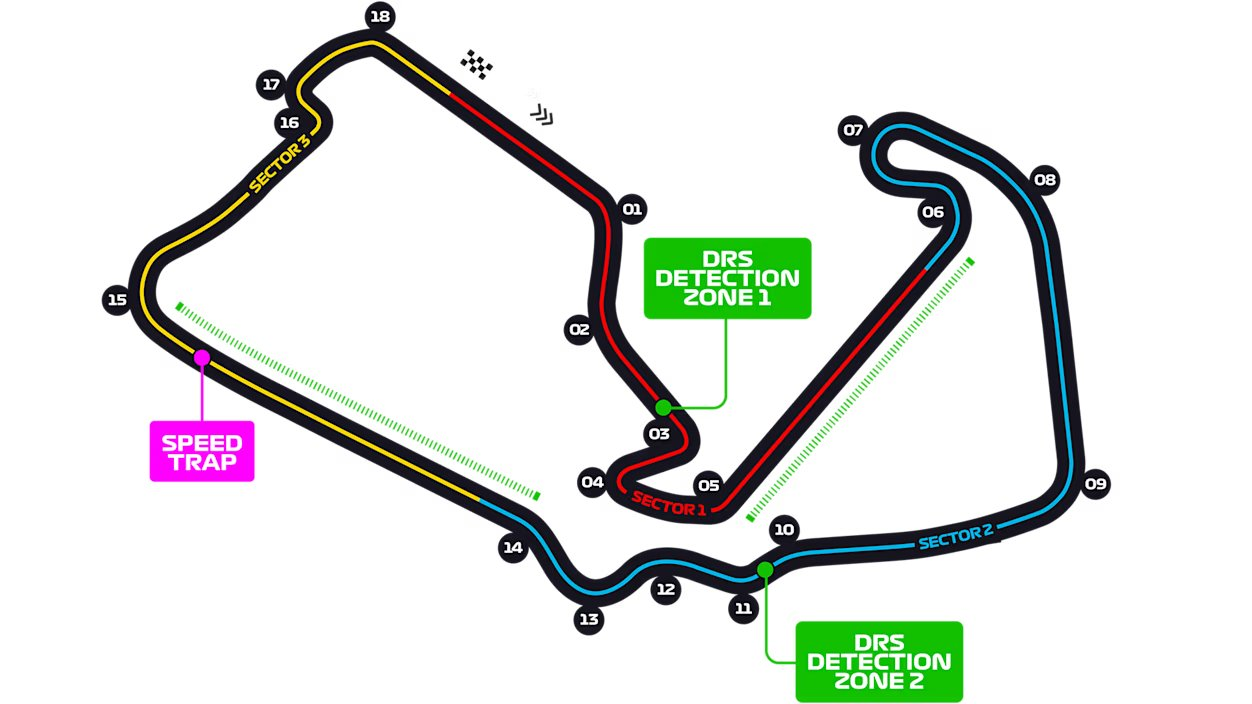
\includegraphics[width=0.75\linewidth]{images/12.Great_Britain_Circuit.jpg}
\end{figure}


\begin{itemize}
    \item \textbf{Lap Record} : 1:25.093 (2017, Lewis Hamilton – Mercedes).
    
    \item \textbf{Number of Corners \& Key Features} : 18 turns (10 right, 8 left) - High-speed classic featuring iconic sections: Maggots–Becketts–Chapel, Copse, Stowe. \\
    Combination of fast corners and technical complexes makes Silverstone a complete car test.
    
    \item \textbf{Braking Zones \& Traction} : Not many heavy braking zones, main ones at Turn 3 (Village) and Turn 16 (Vale).\\
    Traction important out of Club corner onto main straight.

    \item \textbf{DRS \& Overtaking} : Two DRS zones (Wellington straight, Hangar straight).\\
    Main overtaking at Brooklands (Turn 6) and Stowe (Turn 15).
    
    \item \textbf{Tyre Degradation \& Strategy} : High-energy corners stress tyres, especially fronts. Two-stop strategies typical.\\
    Tyre management crucial in long stints.
    
    \item \textbf{Weather \& Environment} : British summer weather often unpredictable: wind, rain possible. Cooler temperatures affect tyre warm-up.
\end{itemize}

\textbf{Strategic Summary :}
Silverstone demands aerodynamic efficiency, high-speed stability, and strong tyre management. 
It is one of the ultimate tests of chassis balance and aerodynamic performance.


\subsection{Race Analysis}

\textbf{Date:} 7 July 2024 — 15:00 local time 

\begin{itemize}
    \item \textbf{Qualifying Summary} : \textbf{Pole Position:} George Russell (Mercedes) – 1:25.819. \\
    Grid: Hamilton 2nd, Norris 3rd, Verstappen 4th.
    
    \item \textbf{Race Summary} : \textbf{Winner:} Lewis Hamilton (Mercedes) - his 104th career victory, first since 2021.\\
    \textbf{Podium:} 1. Hamilton - 2. Verstappen - 3. Norris.\\
    \textbf{Technical issues:} Russell (hydraulic problem).
    
    \item \textbf{Strategies} : 
    - Mercedes: Hamilton on Medium–Inter–Soft, perfectly timed pit windows during rain/slick crossover. \\
    - Red Bull: Verstappen ran Medium–Inter–Hard, lacking late grip vs Hamilton’s softs. \\
    - McLaren: Norris and Piastri delayed stops in changing weather — lost track position. \\
    - Ferrari: Sainz salvaged P5 + fastest lap, Leclerc stuck in midfield with wrong calls. \\
    - Haas: Hülkenberg brilliant P6, maximizing consistency in mixed conditions. \\
    - Aston Martin: Both cars in points (Stroll P7, Alonso P8). \\
    - Williams \& Racing Bulls: Albon P9, Tsunoda P10, opportunistic in changing conditions.
    
    \item \textbf{Performance Trends} : 
    \textbf{Mercedes} delivered their best weekend: Hamilton mastered tyre changes and pressure, Russell unlucky. \\
    \textbf{Red Bull} lacked dominance, Verstappen still consistent with P2. \\
    \textbf{McLaren} had winning pace but strategy errors cost Norris a shot at victory. \\
    \textbf{Ferrari} disappointed, strategy again the weak point. \\
    \textbf{Haas} strong midfield pace, outperforming Aston Martin at times. \\
    \textbf{Williams \& Racing Bulls} scored valuable points, Alpine absent from the fight.
    
    \item \textbf{Championship Impact} : \textbf{Drivers:} Verstappen 255 points, Norris 171, Leclerc 150.\\
    \textbf{Constructors:} Red Bull 373, Ferrari 302, McLaren 295, Mercedes 221.    
\end{itemize}

\textbf{Key Takeaway :}
Hamilton’s masterful tyre management and strategy earned him an emotional home win. Red Bull maintained points lead, McLaren kept momentum, Ferrari slipped back.


\subsection{Link \& Takeaway}

\begin{itemize}
    \item Silverstone’s high-speed corners rewarded Mercedes’ improved aero package, allowing Hamilton to win.
    \item Verstappen and Red Bull remained consistent, but strategy limited their challenge for victory.
    \item McLaren showed podium pace but lacked decisive execution to fight for P1.
    \item Ferrari’s lack of adaptability exposed their weaknesses on high-energy tracks.
    \item Midfield fight remains tight: Haas, Aston Martin, and Williams all capitalized on chaos. 
\end{itemize}